\documentclass[twoside]{book}

% Packages required by doxygen
\usepackage{fixltx2e}
\usepackage{calc}
\usepackage{doxygen}
\usepackage[export]{adjustbox} % also loads graphicx
\usepackage{graphicx}
\usepackage[utf8]{inputenc}
\usepackage{makeidx}
\usepackage{multicol}
\usepackage{multirow}
\PassOptionsToPackage{warn}{textcomp}
\usepackage{textcomp}
\usepackage[nointegrals]{wasysym}
\usepackage[table]{xcolor}

% Font selection
\usepackage[T1]{fontenc}
\usepackage[scaled=.90]{helvet}
\usepackage{courier}
\usepackage{amssymb}
\usepackage{sectsty}
\renewcommand{\familydefault}{\sfdefault}
\allsectionsfont{%
  \fontseries{bc}\selectfont%
  \color{darkgray}%
}
\renewcommand{\DoxyLabelFont}{%
  \fontseries{bc}\selectfont%
  \color{darkgray}%
}
\newcommand{\+}{\discretionary{\mbox{\scriptsize$\hookleftarrow$}}{}{}}

% Page & text layout
\usepackage{geometry}
\geometry{%
  a4paper,%
  top=2.5cm,%
  bottom=2.5cm,%
  left=2.5cm,%
  right=2.5cm%
}
\tolerance=750
\hfuzz=15pt
\hbadness=750
\setlength{\emergencystretch}{15pt}
\setlength{\parindent}{0cm}
\setlength{\parskip}{3ex plus 2ex minus 2ex}
\makeatletter
\renewcommand{\paragraph}{%
  \@startsection{paragraph}{4}{0ex}{-1.0ex}{1.0ex}{%
    \normalfont\normalsize\bfseries\SS@parafont%
  }%
}
\renewcommand{\subparagraph}{%
  \@startsection{subparagraph}{5}{0ex}{-1.0ex}{1.0ex}{%
    \normalfont\normalsize\bfseries\SS@subparafont%
  }%
}
\makeatother

% Headers & footers
\usepackage{fancyhdr}
\pagestyle{fancyplain}
\fancyhead[LE]{\fancyplain{}{\bfseries\thepage}}
\fancyhead[CE]{\fancyplain{}{}}
\fancyhead[RE]{\fancyplain{}{\bfseries\leftmark}}
\fancyhead[LO]{\fancyplain{}{\bfseries\rightmark}}
\fancyhead[CO]{\fancyplain{}{}}
\fancyhead[RO]{\fancyplain{}{\bfseries\thepage}}
\fancyfoot[LE]{\fancyplain{}{}}
\fancyfoot[CE]{\fancyplain{}{}}
\fancyfoot[RE]{\fancyplain{}{\bfseries\scriptsize Generated by Doxygen }}
\fancyfoot[LO]{\fancyplain{}{\bfseries\scriptsize Generated by Doxygen }}
\fancyfoot[CO]{\fancyplain{}{}}
\fancyfoot[RO]{\fancyplain{}{}}
\renewcommand{\footrulewidth}{0.4pt}
\renewcommand{\chaptermark}[1]{%
  \markboth{#1}{}%
}
\renewcommand{\sectionmark}[1]{%
  \markright{\thesection\ #1}%
}

% Indices & bibliography
\usepackage{natbib}
\usepackage[titles]{tocloft}
\setcounter{tocdepth}{3}
\setcounter{secnumdepth}{5}
\makeindex

% Hyperlinks (required, but should be loaded last)
\usepackage{ifpdf}
\ifpdf
  \usepackage[pdftex,pagebackref=true]{hyperref}
\else
  \usepackage[ps2pdf,pagebackref=true]{hyperref}
\fi
\hypersetup{%
  colorlinks=true,%
  linkcolor=blue,%
  citecolor=blue,%
  unicode%
}

% Custom commands
\newcommand{\clearemptydoublepage}{%
  \newpage{\pagestyle{empty}\cleardoublepage}%
}

\usepackage{caption}
\captionsetup{labelsep=space,justification=centering,font={bf},singlelinecheck=off,skip=4pt,position=top}

%===== C O N T E N T S =====

\begin{document}

% Titlepage & ToC
\hypersetup{pageanchor=false,
             bookmarksnumbered=true,
             pdfencoding=unicode
            }
\pagenumbering{alph}
\begin{titlepage}
\vspace*{7cm}
\begin{center}%
{\Large My Project }\\
\vspace*{1cm}
{\large Generated by Doxygen 1.8.14}\\
\end{center}
\end{titlepage}
\clearemptydoublepage
\pagenumbering{roman}
\tableofcontents
\clearemptydoublepage
\pagenumbering{arabic}
\hypersetup{pageanchor=true}

%--- Begin generated contents ---
\chapter{Hierarchical Index}
\section{Class Hierarchy}
This inheritance list is sorted roughly, but not completely, alphabetically\+:\begin{DoxyCompactList}
\item \contentsline{section}{Client}{\pageref{class_client}}{}
\item \contentsline{section}{D\+FS}{\pageref{class_d_f_s}}{}
\item Input\+Stream\begin{DoxyCompactList}
\item \contentsline{section}{File\+Stream}{\pageref{class_file_stream}}{}
\end{DoxyCompactList}
\item \contentsline{section}{Metadata}{\pageref{class_metadata}}{}
\item \contentsline{section}{Meta\+File}{\pageref{class_meta_file}}{}
\item \contentsline{section}{Page}{\pageref{class_page}}{}
\item Remote\begin{DoxyCompactList}
\item \contentsline{section}{Chord\+Message\+Interface}{\pageref{interface_chord_message_interface}}{}
\begin{DoxyCompactList}
\item \contentsline{section}{Chord}{\pageref{class_chord}}{}
\end{DoxyCompactList}
\end{DoxyCompactList}
\item Serializable\begin{DoxyCompactList}
\item \contentsline{section}{File\+Stream}{\pageref{class_file_stream}}{}
\end{DoxyCompactList}
\item Unicast\+Remote\+Object\begin{DoxyCompactList}
\item \contentsline{section}{Chord}{\pageref{class_chord}}{}
\end{DoxyCompactList}
\item \contentsline{section}{User\+Interface}{\pageref{class_user_interface}}{}
\end{DoxyCompactList}

\chapter{Class Index}
\section{Class List}
Here are the classes, structs, unions and interfaces with brief descriptions\+:\begin{DoxyCompactList}
\item\contentsline{section}{\mbox{\hyperlink{class_chord}{Chord}} }{\pageref{class_chord}}{}
\item\contentsline{section}{\mbox{\hyperlink{interface_chord_message_interface}{Chord\+Message\+Interface}} }{\pageref{interface_chord_message_interface}}{}
\item\contentsline{section}{\mbox{\hyperlink{class_client}{Client}} }{\pageref{class_client}}{}
\item\contentsline{section}{\mbox{\hyperlink{class_d_f_s}{D\+FS}} }{\pageref{class_d_f_s}}{}
\item\contentsline{section}{\mbox{\hyperlink{class_file_stream}{File\+Stream}} }{\pageref{class_file_stream}}{}
\item\contentsline{section}{\mbox{\hyperlink{class_metadata}{Metadata}} }{\pageref{class_metadata}}{}
\item\contentsline{section}{\mbox{\hyperlink{class_meta_file}{Meta\+File}} }{\pageref{class_meta_file}}{}
\item\contentsline{section}{\mbox{\hyperlink{class_page}{Page}} }{\pageref{class_page}}{}
\item\contentsline{section}{\mbox{\hyperlink{class_user_interface}{User\+Interface}} }{\pageref{class_user_interface}}{}
\end{DoxyCompactList}

\chapter{Class Documentation}
\hypertarget{class_chord}{}\section{Chord Class Reference}
\label{class_chord}\index{Chord@{Chord}}
Inheritance diagram for Chord\+:\begin{figure}[H]
\begin{center}
\leavevmode
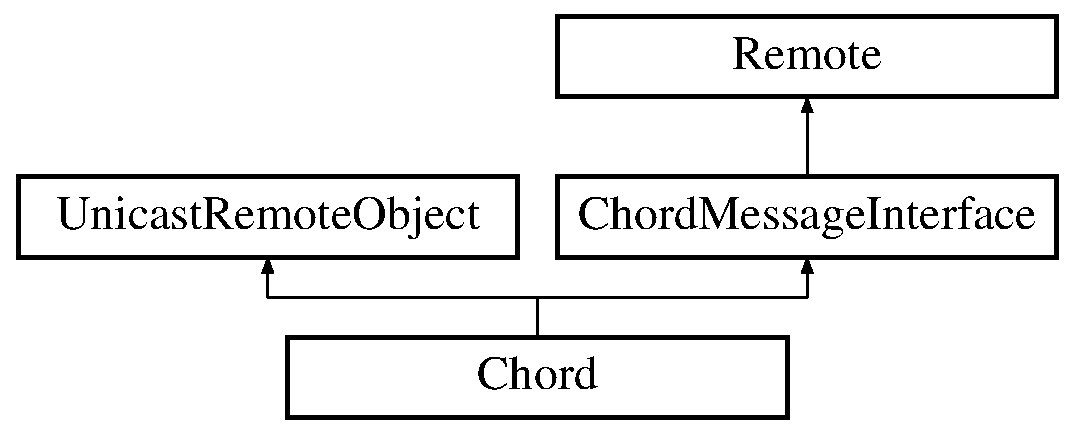
\includegraphics[height=3.000000cm]{class_chord}
\end{center}
\end{figure}
\subsection*{Public Member Functions}
\begin{DoxyCompactItemize}
\item 
\mbox{\Hypertarget{class_chord_aa0b073bf26ea53ee4c36749b5bde4935}\label{class_chord_aa0b073bf26ea53ee4c36749b5bde4935}} 
Boolean {\bfseries is\+Key\+In\+Semi\+Close\+Interval} (long key, long key1, long key2)
\item 
\mbox{\Hypertarget{class_chord_a68c9c3d06da58a6a32aa536751d6a221}\label{class_chord_a68c9c3d06da58a6a32aa536751d6a221}} 
Boolean {\bfseries is\+Key\+In\+Open\+Interval} (long key, long key1, long key2)
\item 
\mbox{\Hypertarget{class_chord_a24d1b07e8c80574244876cf84f86aa4d}\label{class_chord_a24d1b07e8c80574244876cf84f86aa4d}} 
void {\bfseries put} (long guid\+Object, Input\+Stream stream)  throws Remote\+Exception 
\item 
\mbox{\Hypertarget{class_chord_a3e0b4e9a1af09a0604be7eecea716cba}\label{class_chord_a3e0b4e9a1af09a0604be7eecea716cba}} 
Input\+Stream {\bfseries get} (long guid\+Object)  throws Remote\+Exception 
\item 
\mbox{\Hypertarget{class_chord_a8bc6bdc9f92665955ae6907f15cc7ea6}\label{class_chord_a8bc6bdc9f92665955ae6907f15cc7ea6}} 
void {\bfseries delete} (long guid\+Object)  throws Remote\+Exception 
\item 
\mbox{\Hypertarget{class_chord_a3dfb600d109b7d23459a3353af0274a9}\label{class_chord_a3dfb600d109b7d23459a3353af0274a9}} 
long {\bfseries get\+Id} ()  throws Remote\+Exception 
\item 
\mbox{\Hypertarget{class_chord_a0a677ced19cc0cb5afd2a695977aeb95}\label{class_chord_a0a677ced19cc0cb5afd2a695977aeb95}} 
boolean {\bfseries is\+Alive} ()  throws Remote\+Exception 
\item 
\mbox{\Hypertarget{class_chord_a3f1aadce3820e808c80662bb61a58e34}\label{class_chord_a3f1aadce3820e808c80662bb61a58e34}} 
\mbox{\hyperlink{interface_chord_message_interface}{Chord\+Message\+Interface}} {\bfseries get\+Predecessor} ()  throws Remote\+Exception 
\item 
\mbox{\Hypertarget{class_chord_a7e354ea388d048d4910fa28b182ebe9f}\label{class_chord_a7e354ea388d048d4910fa28b182ebe9f}} 
\mbox{\hyperlink{interface_chord_message_interface}{Chord\+Message\+Interface}} {\bfseries locate\+Successor} (long key)  throws Remote\+Exception 
\item 
\mbox{\Hypertarget{class_chord_aecd3971877558c3b1290bd49d7576ab0}\label{class_chord_aecd3971877558c3b1290bd49d7576ab0}} 
\mbox{\hyperlink{interface_chord_message_interface}{Chord\+Message\+Interface}} {\bfseries closest\+Preceding\+Node} (long key)  throws Remote\+Exception 
\item 
\mbox{\Hypertarget{class_chord_ace0b8d2768590d7527af155c6573cae7}\label{class_chord_ace0b8d2768590d7527af155c6573cae7}} 
void {\bfseries join\+Ring} (String ip, int port)  throws Remote\+Exception 
\item 
\mbox{\Hypertarget{class_chord_a65c855dc1d8c6a82545899cb823dba2e}\label{class_chord_a65c855dc1d8c6a82545899cb823dba2e}} 
void {\bfseries finding\+Next\+Successor} ()
\item 
\mbox{\Hypertarget{class_chord_a8a4b7a1cd88cb3f607ada0629f2ff2dd}\label{class_chord_a8a4b7a1cd88cb3f607ada0629f2ff2dd}} 
void {\bfseries stabilize} ()
\item 
\mbox{\Hypertarget{class_chord_a4de8b8464782dd96d88deeb35b2f27a2}\label{class_chord_a4de8b8464782dd96d88deeb35b2f27a2}} 
void {\bfseries notify} (\mbox{\hyperlink{interface_chord_message_interface}{Chord\+Message\+Interface}} j)  throws Remote\+Exception 
\item 
\mbox{\Hypertarget{class_chord_a02763f74bbd986baa7e6567bf9dc3c95}\label{class_chord_a02763f74bbd986baa7e6567bf9dc3c95}} 
void {\bfseries fix\+Fingers} ()
\item 
\mbox{\Hypertarget{class_chord_a530b2ab58c9f4026dadf4293c38c4450}\label{class_chord_a530b2ab58c9f4026dadf4293c38c4450}} 
void {\bfseries check\+Predecessor} ()
\item 
\mbox{\Hypertarget{class_chord_a6e4b3112b0268455fd599c57b5479791}\label{class_chord_a6e4b3112b0268455fd599c57b5479791}} 
{\bfseries Chord} (int port, long guid)  throws Remote\+Exception 
\end{DoxyCompactItemize}
\subsection*{Static Public Attributes}
\begin{DoxyCompactItemize}
\item 
\mbox{\Hypertarget{class_chord_a864e0b4011dc157c78a06dd951c6d9ac}\label{class_chord_a864e0b4011dc157c78a06dd951c6d9ac}} 
static final int {\bfseries M} = 2
\end{DoxyCompactItemize}


The documentation for this class was generated from the following file\+:\begin{DoxyCompactItemize}
\item 
Chord.\+java\end{DoxyCompactItemize}

\hypertarget{interface_chord_message_interface}{}\section{Chord\+Message\+Interface Interface Reference}
\label{interface_chord_message_interface}\index{Chord\+Message\+Interface@{Chord\+Message\+Interface}}
Inheritance diagram for Chord\+Message\+Interface\+:\begin{figure}[H]
\begin{center}
\leavevmode
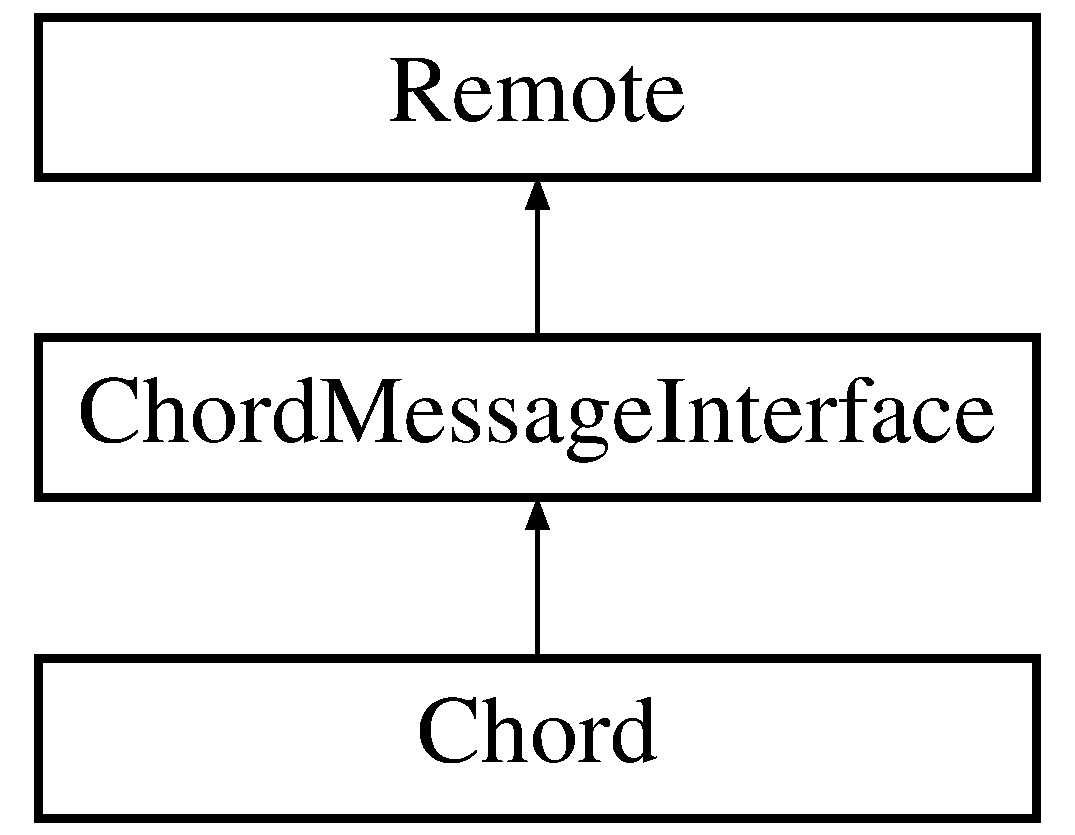
\includegraphics[height=3.000000cm]{interface_chord_message_interface}
\end{center}
\end{figure}
\subsection*{Public Member Functions}
\begin{DoxyCompactItemize}
\item 
\mbox{\Hypertarget{interface_chord_message_interface_ab07c08ba6088ef880eaf4ebae8281c51}\label{interface_chord_message_interface_ab07c08ba6088ef880eaf4ebae8281c51}} 
\mbox{\hyperlink{interface_chord_message_interface}{Chord\+Message\+Interface}} {\bfseries get\+Predecessor} ()  throws Remote\+Exception
\item 
\mbox{\Hypertarget{interface_chord_message_interface_ab7df61ab2cfee0f39206014d7a42b063}\label{interface_chord_message_interface_ab7df61ab2cfee0f39206014d7a42b063}} 
\mbox{\hyperlink{interface_chord_message_interface}{Chord\+Message\+Interface}} {\bfseries locate\+Successor} (long key)  throws Remote\+Exception
\item 
\mbox{\Hypertarget{interface_chord_message_interface_a1d54a4ccd64382455af7dccfd0d6f95f}\label{interface_chord_message_interface_a1d54a4ccd64382455af7dccfd0d6f95f}} 
\mbox{\hyperlink{interface_chord_message_interface}{Chord\+Message\+Interface}} {\bfseries closest\+Preceding\+Node} (long key)  throws Remote\+Exception
\item 
\mbox{\Hypertarget{interface_chord_message_interface_abc5a9483416a6b8ae7330b324869e236}\label{interface_chord_message_interface_abc5a9483416a6b8ae7330b324869e236}} 
void {\bfseries join\+Ring} (String Ip, int port)  throws Remote\+Exception
\item 
\mbox{\Hypertarget{interface_chord_message_interface_abbb77f94541073d79284d35f970e0eb4}\label{interface_chord_message_interface_abbb77f94541073d79284d35f970e0eb4}} 
void {\bfseries notify} (\mbox{\hyperlink{interface_chord_message_interface}{Chord\+Message\+Interface}} j)  throws Remote\+Exception
\item 
\mbox{\Hypertarget{interface_chord_message_interface_a8165b3fb53905e657c70b66223197561}\label{interface_chord_message_interface_a8165b3fb53905e657c70b66223197561}} 
boolean {\bfseries is\+Alive} ()  throws Remote\+Exception
\item 
\mbox{\Hypertarget{interface_chord_message_interface_aaa28e7b91333c557955404ee8d26d65a}\label{interface_chord_message_interface_aaa28e7b91333c557955404ee8d26d65a}} 
long {\bfseries get\+Id} ()  throws Remote\+Exception
\item 
\mbox{\Hypertarget{interface_chord_message_interface_a0731e7364624abf44be7ddb7a0d34341}\label{interface_chord_message_interface_a0731e7364624abf44be7ddb7a0d34341}} 
void {\bfseries put} (long guid\+Object, Input\+Stream input\+Stream)  throws I\+O\+Exception, Remote\+Exception
\item 
\mbox{\Hypertarget{interface_chord_message_interface_ad25e17fc24b4204afb6af590922bae5a}\label{interface_chord_message_interface_ad25e17fc24b4204afb6af590922bae5a}} 
Input\+Stream {\bfseries get} (long guid\+Object)  throws I\+O\+Exception, Remote\+Exception
\item 
\mbox{\Hypertarget{interface_chord_message_interface_a2bd41258d7f62c5959907e4d3170fc70}\label{interface_chord_message_interface_a2bd41258d7f62c5959907e4d3170fc70}} 
void {\bfseries delete} (long guid\+Object)  throws I\+O\+Exception, Remote\+Exception
\end{DoxyCompactItemize}


The documentation for this interface was generated from the following file\+:\begin{DoxyCompactItemize}
\item 
Chord\+Message\+Interface.\+java\end{DoxyCompactItemize}

\hypertarget{class_client}{}\section{Client Class Reference}
\label{class_client}\index{Client@{Client}}
\subsection*{Public Member Functions}
\begin{DoxyCompactItemize}
\item 
\mbox{\Hypertarget{class_client_a1862ab048047a5917b5e6a01bf38b78e}\label{class_client_a1862ab048047a5917b5e6a01bf38b78e}} 
{\bfseries Client} (int port)  throws Exception 
\end{DoxyCompactItemize}
\subsection*{Static Public Member Functions}
\begin{DoxyCompactItemize}
\item 
\mbox{\Hypertarget{class_client_ac4219c51358857184ceeb023ada3d8ae}\label{class_client_ac4219c51358857184ceeb023ada3d8ae}} 
static void {\bfseries main} (String args\mbox{[}$\,$\mbox{]})  throws Exception     
\end{DoxyCompactItemize}


The documentation for this class was generated from the following file\+:\begin{DoxyCompactItemize}
\item 
Client.\+java\end{DoxyCompactItemize}

\hypertarget{class_d_f_s}{}\section{D\+FS Class Reference}
\label{class_d_f_s}\index{D\+FS@{D\+FS}}
\subsection*{Public Member Functions}
\begin{DoxyCompactItemize}
\item 
\mbox{\hyperlink{class_d_f_s_ad863806217afcce82e64f5d7d4c124ad}{D\+FS}} (int port)  throws Exception     
\item 
\mbox{\Hypertarget{class_d_f_s_afb27b3ac552ee5a0b615f76157ebde81}\label{class_d_f_s_afb27b3ac552ee5a0b615f76157ebde81}} 
void {\bfseries join} (String Ip, int port)  throws Exception 
\item 
void \mbox{\hyperlink{class_d_f_s_a7b0d44e11c6176a71d040919b6fe1d96}{mv}} (String old\+Name, String new\+Name)  throws Exception 
\item 
String \mbox{\hyperlink{class_d_f_s_a753e09aab8e500f333585f1a6ee865e1}{ls}} ()  throws Exception 
\item 
void \mbox{\hyperlink{class_d_f_s_ac44bf8288f4423fc87370b97f95f07c1}{touch}} (String file\+Name)  throws Exception 
\item 
void \mbox{\hyperlink{class_d_f_s_afa4df78a9af4f942cd878afc329b98e1}{delete}} (String file\+Name)  throws Exception 
\item 
\mbox{\hyperlink{class_file_stream}{File\+Stream}} \mbox{\hyperlink{class_d_f_s_a2fe4f98b6e0dede1c97d67bbb5c77df1}{read}} (String file\+Name, int page\+Number)  throws Exception     
\item 
\mbox{\hyperlink{class_file_stream}{File\+Stream}} \mbox{\hyperlink{class_d_f_s_a86ed64f3b14dc0c0d878dbcb1ca1cfa9}{tail}} (String file\+Name)  throws Exception     
\item 
\mbox{\hyperlink{class_file_stream}{File\+Stream}} \mbox{\hyperlink{class_d_f_s_a73915159a4290c3832635b6c4338ff7e}{head}} (String file\+Name)  throws Exception     
\item 
void \mbox{\hyperlink{class_d_f_s_a119519b72f38226815a4b65760701dcf}{append}} (String filename, String filepath)  throws Exception     
\end{DoxyCompactItemize}


\subsection{Constructor \& Destructor Documentation}
\mbox{\Hypertarget{class_d_f_s_ad863806217afcce82e64f5d7d4c124ad}\label{class_d_f_s_ad863806217afcce82e64f5d7d4c124ad}} 
\index{D\+FS@{D\+FS}!D\+FS@{D\+FS}}
\index{D\+FS@{D\+FS}!D\+FS@{D\+FS}}
\subsubsection{\texorpdfstring{D\+F\+S()}{DFS()}}
{\footnotesize\ttfamily D\+F\+S.\+D\+FS (\begin{DoxyParamCaption}\item[{int}]{port }\end{DoxyParamCaption}) throws Exception\hspace{0.3cm}{\ttfamily [inline]}}

Constructor for the \mbox{\hyperlink{class_d_f_s}{D\+FS}} class. Takes an integer as the port number. 
\begin{DoxyParams}{Parameters}
{\em port} & \\
\hline
\end{DoxyParams}

\begin{DoxyExceptions}{Exceptions}
{\em Exception} & \\
\hline
\end{DoxyExceptions}


\subsection{Member Function Documentation}
\mbox{\Hypertarget{class_d_f_s_a119519b72f38226815a4b65760701dcf}\label{class_d_f_s_a119519b72f38226815a4b65760701dcf}} 
\index{D\+FS@{D\+FS}!append@{append}}
\index{append@{append}!D\+FS@{D\+FS}}
\subsubsection{\texorpdfstring{append()}{append()}}
{\footnotesize\ttfamily void D\+F\+S.\+append (\begin{DoxyParamCaption}\item[{String}]{filename,  }\item[{String}]{filepath }\end{DoxyParamCaption}) throws Exception\hspace{0.3cm}{\ttfamily [inline]}}

Adds a new file to the end of the array of files in the metadata. 
\begin{DoxyParams}{Parameters}
{\em filename} & \\
\hline
{\em filepath} & \\
\hline
\end{DoxyParams}

\begin{DoxyExceptions}{Exceptions}
{\em Exception} & \\
\hline
\end{DoxyExceptions}
\mbox{\Hypertarget{class_d_f_s_afa4df78a9af4f942cd878afc329b98e1}\label{class_d_f_s_afa4df78a9af4f942cd878afc329b98e1}} 
\index{D\+FS@{D\+FS}!delete@{delete}}
\index{delete@{delete}!D\+FS@{D\+FS}}
\subsubsection{\texorpdfstring{delete()}{delete()}}
{\footnotesize\ttfamily void D\+F\+S.\+delete (\begin{DoxyParamCaption}\item[{String}]{file\+Name }\end{DoxyParamCaption}) throws Exception\hspace{0.3cm}{\ttfamily [inline]}}

Deletes a file and all of its pages from the metadata. 
\begin{DoxyParams}{Parameters}
{\em file\+Name} & \\
\hline
\end{DoxyParams}

\begin{DoxyExceptions}{Exceptions}
{\em Exception} & \\
\hline
\end{DoxyExceptions}
\mbox{\Hypertarget{class_d_f_s_a73915159a4290c3832635b6c4338ff7e}\label{class_d_f_s_a73915159a4290c3832635b6c4338ff7e}} 
\index{D\+FS@{D\+FS}!head@{head}}
\index{head@{head}!D\+FS@{D\+FS}}
\subsubsection{\texorpdfstring{head()}{head()}}
{\footnotesize\ttfamily \mbox{\hyperlink{class_file_stream}{File\+Stream}} D\+F\+S.\+head (\begin{DoxyParamCaption}\item[{String}]{file\+Name }\end{DoxyParamCaption}) throws Exception\hspace{0.3cm}{\ttfamily [inline]}}

Returns the first page of the file in the metadata. 
\begin{DoxyParams}{Parameters}
{\em file\+Name} & \\
\hline
\end{DoxyParams}
\begin{DoxyReturn}{Returns}

\end{DoxyReturn}

\begin{DoxyExceptions}{Exceptions}
{\em Exception} & \\
\hline
\end{DoxyExceptions}
\mbox{\Hypertarget{class_d_f_s_a753e09aab8e500f333585f1a6ee865e1}\label{class_d_f_s_a753e09aab8e500f333585f1a6ee865e1}} 
\index{D\+FS@{D\+FS}!ls@{ls}}
\index{ls@{ls}!D\+FS@{D\+FS}}
\subsubsection{\texorpdfstring{ls()}{ls()}}
{\footnotesize\ttfamily String D\+F\+S.\+ls (\begin{DoxyParamCaption}{ }\end{DoxyParamCaption}) throws Exception\hspace{0.3cm}{\ttfamily [inline]}}

Returns a list of the files in the metadata in the form of a string. \begin{DoxyReturn}{Returns}

\end{DoxyReturn}

\begin{DoxyExceptions}{Exceptions}
{\em Exception} & \\
\hline
\end{DoxyExceptions}
\mbox{\Hypertarget{class_d_f_s_a7b0d44e11c6176a71d040919b6fe1d96}\label{class_d_f_s_a7b0d44e11c6176a71d040919b6fe1d96}} 
\index{D\+FS@{D\+FS}!mv@{mv}}
\index{mv@{mv}!D\+FS@{D\+FS}}
\subsubsection{\texorpdfstring{mv()}{mv()}}
{\footnotesize\ttfamily void D\+F\+S.\+mv (\begin{DoxyParamCaption}\item[{String}]{old\+Name,  }\item[{String}]{new\+Name }\end{DoxyParamCaption}) throws Exception\hspace{0.3cm}{\ttfamily [inline]}}

Renames the metadata object. 
\begin{DoxyParams}{Parameters}
{\em old\+Name} & \\
\hline
{\em new\+Name} & \\
\hline
\end{DoxyParams}

\begin{DoxyExceptions}{Exceptions}
{\em Exception} & \\
\hline
\end{DoxyExceptions}
\mbox{\Hypertarget{class_d_f_s_a2fe4f98b6e0dede1c97d67bbb5c77df1}\label{class_d_f_s_a2fe4f98b6e0dede1c97d67bbb5c77df1}} 
\index{D\+FS@{D\+FS}!read@{read}}
\index{read@{read}!D\+FS@{D\+FS}}
\subsubsection{\texorpdfstring{read()}{read()}}
{\footnotesize\ttfamily \mbox{\hyperlink{class_file_stream}{File\+Stream}} D\+F\+S.\+read (\begin{DoxyParamCaption}\item[{String}]{file\+Name,  }\item[{int}]{page\+Number }\end{DoxyParamCaption}) throws Exception\hspace{0.3cm}{\ttfamily [inline]}}

Returns a page from a file from the metadata in the form of a \mbox{\hyperlink{class_file_stream}{File\+Stream}}. 
\begin{DoxyParams}{Parameters}
{\em file\+Name} & \\
\hline
{\em page\+Number} & \\
\hline
\end{DoxyParams}
\begin{DoxyReturn}{Returns}

\end{DoxyReturn}

\begin{DoxyExceptions}{Exceptions}
{\em Exception} & \\
\hline
\end{DoxyExceptions}
\mbox{\Hypertarget{class_d_f_s_a86ed64f3b14dc0c0d878dbcb1ca1cfa9}\label{class_d_f_s_a86ed64f3b14dc0c0d878dbcb1ca1cfa9}} 
\index{D\+FS@{D\+FS}!tail@{tail}}
\index{tail@{tail}!D\+FS@{D\+FS}}
\subsubsection{\texorpdfstring{tail()}{tail()}}
{\footnotesize\ttfamily \mbox{\hyperlink{class_file_stream}{File\+Stream}} D\+F\+S.\+tail (\begin{DoxyParamCaption}\item[{String}]{file\+Name }\end{DoxyParamCaption}) throws Exception\hspace{0.3cm}{\ttfamily [inline]}}

Returns the last page of a file in the metadata in the form of a Filestream. 
\begin{DoxyParams}{Parameters}
{\em file\+Name} & \\
\hline
\end{DoxyParams}
\begin{DoxyReturn}{Returns}
Filestream 
\end{DoxyReturn}

\begin{DoxyExceptions}{Exceptions}
{\em Exception} & \\
\hline
\end{DoxyExceptions}
\mbox{\Hypertarget{class_d_f_s_ac44bf8288f4423fc87370b97f95f07c1}\label{class_d_f_s_ac44bf8288f4423fc87370b97f95f07c1}} 
\index{D\+FS@{D\+FS}!touch@{touch}}
\index{touch@{touch}!D\+FS@{D\+FS}}
\subsubsection{\texorpdfstring{touch()}{touch()}}
{\footnotesize\ttfamily void D\+F\+S.\+touch (\begin{DoxyParamCaption}\item[{String}]{file\+Name }\end{DoxyParamCaption}) throws Exception\hspace{0.3cm}{\ttfamily [inline]}}

Creates a new file with the inputted name into the metadata object. 
\begin{DoxyParams}{Parameters}
{\em file\+Name} & \\
\hline
\end{DoxyParams}

\begin{DoxyExceptions}{Exceptions}
{\em Exception} & \\
\hline
\end{DoxyExceptions}


The documentation for this class was generated from the following file\+:\begin{DoxyCompactItemize}
\item 
D\+F\+S.\+java\end{DoxyCompactItemize}

\hypertarget{class_file_stream}{}\section{File\+Stream Class Reference}
\label{class_file_stream}\index{File\+Stream@{File\+Stream}}
Inheritance diagram for File\+Stream\+:\begin{figure}[H]
\begin{center}
\leavevmode
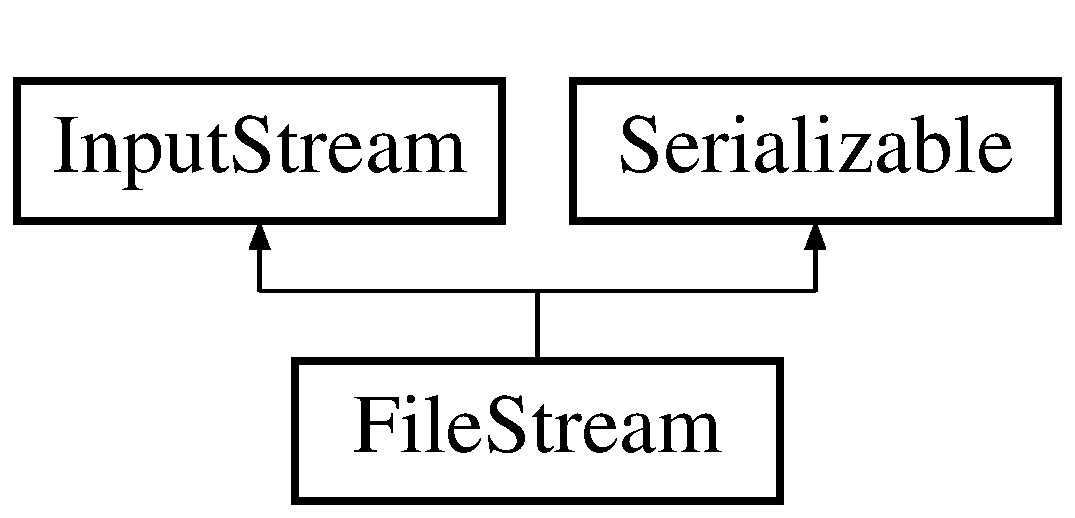
\includegraphics[height=2.000000cm]{class_file_stream}
\end{center}
\end{figure}
\subsection*{Public Member Functions}
\begin{DoxyCompactItemize}
\item 
\mbox{\Hypertarget{class_file_stream_a120b1fd6e4c74e93199d063da1c65b98}\label{class_file_stream_a120b1fd6e4c74e93199d063da1c65b98}} 
{\bfseries File\+Stream} (String path\+Name)  throws File\+Not\+Found\+Exception, I\+O\+Exception    
\item 
\mbox{\Hypertarget{class_file_stream_a7f2ea40eff2241931a4ca971364cd532}\label{class_file_stream_a7f2ea40eff2241931a4ca971364cd532}} 
int {\bfseries read} ()  throws I\+O\+Exception 
\item 
\mbox{\Hypertarget{class_file_stream_a7dd240b96afa9e37f9a6bd8e4b99e48b}\label{class_file_stream_a7dd240b96afa9e37f9a6bd8e4b99e48b}} 
int {\bfseries available} ()  throws I\+O\+Exception     
\item 
\mbox{\Hypertarget{class_file_stream_ab8f4d0c94a6c1357c7af77a4121e52fc}\label{class_file_stream_ab8f4d0c94a6c1357c7af77a4121e52fc}} 
int {\bfseries get\+Size} ()
\end{DoxyCompactItemize}


The documentation for this class was generated from the following file\+:\begin{DoxyCompactItemize}
\item 
File\+Stream.\+java\end{DoxyCompactItemize}

\hypertarget{class_metadata}{}\section{Metadata Class Reference}
\label{class_metadata}\index{Metadata@{Metadata}}
\subsection*{Public Member Functions}
\begin{DoxyCompactItemize}
\item 
\mbox{\hyperlink{class_metadata_a5d0290e9e1427f229a976d921da5423b}{Metadata}} (String name, Array\+List$<$ \mbox{\hyperlink{class_meta_file}{Meta\+File}} $>$ metafiles)
\item 
void \mbox{\hyperlink{class_metadata_ad82a2024da7159b62b4baaf431c986e6}{change\+Name}} (String newname)
\item 
String \mbox{\hyperlink{class_metadata_a47932985a21ca5fe3e99726b50c36658}{get\+File\+Names}} ()
\item 
void \mbox{\hyperlink{class_metadata_a67800e2f003cabb15744b86bec38a783}{create\+File}} (String file\+Name)
\item 
\mbox{\hyperlink{class_meta_file}{Meta\+File}} \mbox{\hyperlink{class_metadata_ae29cb4e7e73fdda5a3649e085863d481}{get\+File}} (String file\+Name)  throws Exception 	
\item 
\mbox{\Hypertarget{class_metadata_ad553fd3bd0610354c55d603c64886533}\label{class_metadata_ad553fd3bd0610354c55d603c64886533}} 
void {\bfseries to\+Json} ()
\item 
\mbox{\Hypertarget{class_metadata_ab22a1ff2f8390792d6c520be50dd3906}\label{class_metadata_ab22a1ff2f8390792d6c520be50dd3906}} 
void {\bfseries readfrom\+J\+S\+ON} ()
\item 
\mbox{\Hypertarget{class_metadata_a8176cc867722d5a71d2a17ba574d61bc}\label{class_metadata_a8176cc867722d5a71d2a17ba574d61bc}} 
void {\bfseries delete\+File} ()
\end{DoxyCompactItemize}


\subsection{Constructor \& Destructor Documentation}
\mbox{\Hypertarget{class_metadata_a5d0290e9e1427f229a976d921da5423b}\label{class_metadata_a5d0290e9e1427f229a976d921da5423b}} 
\index{Metadata@{Metadata}!Metadata@{Metadata}}
\index{Metadata@{Metadata}!Metadata@{Metadata}}
\subsubsection{\texorpdfstring{Metadata()}{Metadata()}}
{\footnotesize\ttfamily Metadata.\+Metadata (\begin{DoxyParamCaption}\item[{String}]{name,  }\item[{Array\+List$<$ \mbox{\hyperlink{class_meta_file}{Meta\+File}} $>$}]{metafiles }\end{DoxyParamCaption})\hspace{0.3cm}{\ttfamily [inline]}}

Constructor for the metadata class. Requires a string name and an arraylist of files. 
\begin{DoxyParams}{Parameters}
{\em name} & \\
\hline
{\em metafiles} & \\
\hline
\end{DoxyParams}


\subsection{Member Function Documentation}
\mbox{\Hypertarget{class_metadata_ad82a2024da7159b62b4baaf431c986e6}\label{class_metadata_ad82a2024da7159b62b4baaf431c986e6}} 
\index{Metadata@{Metadata}!change\+Name@{change\+Name}}
\index{change\+Name@{change\+Name}!Metadata@{Metadata}}
\subsubsection{\texorpdfstring{change\+Name()}{changeName()}}
{\footnotesize\ttfamily void Metadata.\+change\+Name (\begin{DoxyParamCaption}\item[{String}]{newname }\end{DoxyParamCaption})\hspace{0.3cm}{\ttfamily [inline]}}

Renames the metadata\textquotesingle{}s name with a new one. 
\begin{DoxyParams}{Parameters}
{\em newname} & \\
\hline
\end{DoxyParams}
\mbox{\Hypertarget{class_metadata_a67800e2f003cabb15744b86bec38a783}\label{class_metadata_a67800e2f003cabb15744b86bec38a783}} 
\index{Metadata@{Metadata}!create\+File@{create\+File}}
\index{create\+File@{create\+File}!Metadata@{Metadata}}
\subsubsection{\texorpdfstring{create\+File()}{createFile()}}
{\footnotesize\ttfamily void Metadata.\+create\+File (\begin{DoxyParamCaption}\item[{String}]{file\+Name }\end{DoxyParamCaption})\hspace{0.3cm}{\ttfamily [inline]}}


\begin{DoxyParams}{Parameters}
{\em file\+Name} & \\
\hline
\end{DoxyParams}
\mbox{\Hypertarget{class_metadata_ae29cb4e7e73fdda5a3649e085863d481}\label{class_metadata_ae29cb4e7e73fdda5a3649e085863d481}} 
\index{Metadata@{Metadata}!get\+File@{get\+File}}
\index{get\+File@{get\+File}!Metadata@{Metadata}}
\subsubsection{\texorpdfstring{get\+File()}{getFile()}}
{\footnotesize\ttfamily \mbox{\hyperlink{class_meta_file}{Meta\+File}} Metadata.\+get\+File (\begin{DoxyParamCaption}\item[{String}]{file\+Name }\end{DoxyParamCaption}) throws Exception\hspace{0.3cm}{\ttfamily [inline]}}

Returns a specific file using the filename inputted. 
\begin{DoxyParams}{Parameters}
{\em file\+Name} & \\
\hline
\end{DoxyParams}
\begin{DoxyReturn}{Returns}

\end{DoxyReturn}

\begin{DoxyExceptions}{Exceptions}
{\em Exception} & \\
\hline
\end{DoxyExceptions}
\mbox{\Hypertarget{class_metadata_a47932985a21ca5fe3e99726b50c36658}\label{class_metadata_a47932985a21ca5fe3e99726b50c36658}} 
\index{Metadata@{Metadata}!get\+File\+Names@{get\+File\+Names}}
\index{get\+File\+Names@{get\+File\+Names}!Metadata@{Metadata}}
\subsubsection{\texorpdfstring{get\+File\+Names()}{getFileNames()}}
{\footnotesize\ttfamily String Metadata.\+get\+File\+Names (\begin{DoxyParamCaption}{ }\end{DoxyParamCaption})\hspace{0.3cm}{\ttfamily [inline]}}

Returns a list of all of the file\textquotesingle{}s names in the form of a string. \begin{DoxyReturn}{Returns}

\end{DoxyReturn}


The documentation for this class was generated from the following file\+:\begin{DoxyCompactItemize}
\item 
Metadata.\+java\end{DoxyCompactItemize}

\hypertarget{class_meta_file}{}\section{Meta\+File Class Reference}
\label{class_meta_file}\index{Meta\+File@{Meta\+File}}
\subsection*{Public Member Functions}
\begin{DoxyCompactItemize}
\item 
\mbox{\hyperlink{class_meta_file_aa0e71eb6d56f1e50c2cf53c321a7b4c0}{Meta\+File}} (String name, int number\+Of\+Pages, int page\+Size, int size, Array\+List$<$ \mbox{\hyperlink{class_page}{Page}} $>$ pages)
\item 
String \mbox{\hyperlink{class_meta_file_a7704cca7da5d2e765d70d01562d6f4da}{get\+Name}} ()
\item 
\mbox{\hyperlink{class_page}{Page}} \mbox{\hyperlink{class_meta_file_a28c7cbf3f8889b484df5b11b99825a4e}{get\+Page}} (int page\+Num)  throws Exception 	
\item 
void \mbox{\hyperlink{class_meta_file_ad8fc179c2db8ceee473dbcd833d5a7bd}{add\+Page}} (\mbox{\hyperlink{class_page}{Page}} page)
\item 
\mbox{\hyperlink{class_page}{Page}} \mbox{\hyperlink{class_meta_file_adf3ad8347572a056d3a7ae730c120303}{get\+Last\+Page}} ()
\item 
\mbox{\hyperlink{class_page}{Page}} \mbox{\hyperlink{class_meta_file_a495f8b327a312ebcdd54e7dbfdd98ee5}{get\+First\+Page}} ()
\end{DoxyCompactItemize}


\subsection{Constructor \& Destructor Documentation}
\mbox{\Hypertarget{class_meta_file_aa0e71eb6d56f1e50c2cf53c321a7b4c0}\label{class_meta_file_aa0e71eb6d56f1e50c2cf53c321a7b4c0}} 
\index{Meta\+File@{Meta\+File}!Meta\+File@{Meta\+File}}
\index{Meta\+File@{Meta\+File}!Meta\+File@{Meta\+File}}
\subsubsection{\texorpdfstring{Meta\+File()}{MetaFile()}}
{\footnotesize\ttfamily Meta\+File.\+Meta\+File (\begin{DoxyParamCaption}\item[{String}]{name,  }\item[{int}]{number\+Of\+Pages,  }\item[{int}]{page\+Size,  }\item[{int}]{size,  }\item[{Array\+List$<$ \mbox{\hyperlink{class_page}{Page}} $>$}]{pages }\end{DoxyParamCaption})\hspace{0.3cm}{\ttfamily [inline]}}

Constructor for the \mbox{\hyperlink{class_meta_file}{Meta\+File}} class. Requires a name, the number of pages, the page size, file size, and an arraylist of pages. 
\begin{DoxyParams}{Parameters}
{\em name} & \\
\hline
{\em number\+Of\+Pages} & \\
\hline
{\em page\+Size} & \\
\hline
{\em size} & \\
\hline
{\em pages} & \\
\hline
\end{DoxyParams}


\subsection{Member Function Documentation}
\mbox{\Hypertarget{class_meta_file_ad8fc179c2db8ceee473dbcd833d5a7bd}\label{class_meta_file_ad8fc179c2db8ceee473dbcd833d5a7bd}} 
\index{Meta\+File@{Meta\+File}!add\+Page@{add\+Page}}
\index{add\+Page@{add\+Page}!Meta\+File@{Meta\+File}}
\subsubsection{\texorpdfstring{add\+Page()}{addPage()}}
{\footnotesize\ttfamily void Meta\+File.\+add\+Page (\begin{DoxyParamCaption}\item[{\mbox{\hyperlink{class_page}{Page}}}]{page }\end{DoxyParamCaption})\hspace{0.3cm}{\ttfamily [inline]}}

Appends a page to the arraylist of pages. 
\begin{DoxyParams}{Parameters}
{\em page} & \\
\hline
\end{DoxyParams}
\mbox{\Hypertarget{class_meta_file_a495f8b327a312ebcdd54e7dbfdd98ee5}\label{class_meta_file_a495f8b327a312ebcdd54e7dbfdd98ee5}} 
\index{Meta\+File@{Meta\+File}!get\+First\+Page@{get\+First\+Page}}
\index{get\+First\+Page@{get\+First\+Page}!Meta\+File@{Meta\+File}}
\subsubsection{\texorpdfstring{get\+First\+Page()}{getFirstPage()}}
{\footnotesize\ttfamily \mbox{\hyperlink{class_page}{Page}} Meta\+File.\+get\+First\+Page (\begin{DoxyParamCaption}{ }\end{DoxyParamCaption})\hspace{0.3cm}{\ttfamily [inline]}}

Returns the first page in the array. \begin{DoxyReturn}{Returns}

\end{DoxyReturn}
\mbox{\Hypertarget{class_meta_file_adf3ad8347572a056d3a7ae730c120303}\label{class_meta_file_adf3ad8347572a056d3a7ae730c120303}} 
\index{Meta\+File@{Meta\+File}!get\+Last\+Page@{get\+Last\+Page}}
\index{get\+Last\+Page@{get\+Last\+Page}!Meta\+File@{Meta\+File}}
\subsubsection{\texorpdfstring{get\+Last\+Page()}{getLastPage()}}
{\footnotesize\ttfamily \mbox{\hyperlink{class_page}{Page}} Meta\+File.\+get\+Last\+Page (\begin{DoxyParamCaption}{ }\end{DoxyParamCaption})\hspace{0.3cm}{\ttfamily [inline]}}

Returns the last page in the array. \begin{DoxyReturn}{Returns}

\end{DoxyReturn}
\mbox{\Hypertarget{class_meta_file_a7704cca7da5d2e765d70d01562d6f4da}\label{class_meta_file_a7704cca7da5d2e765d70d01562d6f4da}} 
\index{Meta\+File@{Meta\+File}!get\+Name@{get\+Name}}
\index{get\+Name@{get\+Name}!Meta\+File@{Meta\+File}}
\subsubsection{\texorpdfstring{get\+Name()}{getName()}}
{\footnotesize\ttfamily String Meta\+File.\+get\+Name (\begin{DoxyParamCaption}{ }\end{DoxyParamCaption})\hspace{0.3cm}{\ttfamily [inline]}}

Returns the name of the metafile. \begin{DoxyReturn}{Returns}

\end{DoxyReturn}
\mbox{\Hypertarget{class_meta_file_a28c7cbf3f8889b484df5b11b99825a4e}\label{class_meta_file_a28c7cbf3f8889b484df5b11b99825a4e}} 
\index{Meta\+File@{Meta\+File}!get\+Page@{get\+Page}}
\index{get\+Page@{get\+Page}!Meta\+File@{Meta\+File}}
\subsubsection{\texorpdfstring{get\+Page()}{getPage()}}
{\footnotesize\ttfamily \mbox{\hyperlink{class_page}{Page}} Meta\+File.\+get\+Page (\begin{DoxyParamCaption}\item[{int}]{page\+Num }\end{DoxyParamCaption}) throws Exception\hspace{0.3cm}{\ttfamily [inline]}}

Returns the specified page from the inputted number. 
\begin{DoxyParams}{Parameters}
{\em page\+Num} & \\
\hline
\end{DoxyParams}
\begin{DoxyReturn}{Returns}

\end{DoxyReturn}

\begin{DoxyExceptions}{Exceptions}
{\em Exception} & \\
\hline
\end{DoxyExceptions}


The documentation for this class was generated from the following file\+:\begin{DoxyCompactItemize}
\item 
Meta\+File.\+java\end{DoxyCompactItemize}

\hypertarget{class_page}{}\section{Page Class Reference}
\label{class_page}\index{Page@{Page}}
\subsection*{Public Member Functions}
\begin{DoxyCompactItemize}
\item 
\mbox{\hyperlink{class_page_a2ab2c53a979db9210921dc1ae1748008}{Page}} (int number, long guid, long size)
\item 
int \mbox{\hyperlink{class_page_abbbbf34472bff8012ba88bc10a8739fa}{get\+Number}} ()
\end{DoxyCompactItemize}


\subsection{Constructor \& Destructor Documentation}
\mbox{\Hypertarget{class_page_a2ab2c53a979db9210921dc1ae1748008}\label{class_page_a2ab2c53a979db9210921dc1ae1748008}} 
\index{Page@{Page}!Page@{Page}}
\index{Page@{Page}!Page@{Page}}
\subsubsection{\texorpdfstring{Page()}{Page()}}
{\footnotesize\ttfamily Page.\+Page (\begin{DoxyParamCaption}\item[{int}]{number,  }\item[{long}]{guid,  }\item[{long}]{size }\end{DoxyParamCaption})\hspace{0.3cm}{\ttfamily [inline]}}

The constructor for the page class. Requires a page number, a guid, and the page size. 
\begin{DoxyParams}{Parameters}
{\em number} & \\
\hline
{\em guid} & \\
\hline
{\em size} & \\
\hline
\end{DoxyParams}


\subsection{Member Function Documentation}
\mbox{\Hypertarget{class_page_abbbbf34472bff8012ba88bc10a8739fa}\label{class_page_abbbbf34472bff8012ba88bc10a8739fa}} 
\index{Page@{Page}!get\+Number@{get\+Number}}
\index{get\+Number@{get\+Number}!Page@{Page}}
\subsubsection{\texorpdfstring{get\+Number()}{getNumber()}}
{\footnotesize\ttfamily int Page.\+get\+Number (\begin{DoxyParamCaption}{ }\end{DoxyParamCaption})\hspace{0.3cm}{\ttfamily [inline]}}

Returns the page\textquotesingle{}s number. \begin{DoxyReturn}{Returns}

\end{DoxyReturn}


The documentation for this class was generated from the following file\+:\begin{DoxyCompactItemize}
\item 
Page.\+java\end{DoxyCompactItemize}

\hypertarget{class_user_interface}{}\section{User\+Interface Class Reference}
\label{class_user_interface}\index{User\+Interface@{User\+Interface}}
\subsection*{Public Member Functions}
\begin{DoxyCompactItemize}
\item 
\mbox{\hyperlink{class_user_interface_ae4be0a3dc956ead335dbb0c627847b1f}{User\+Interface}} (\mbox{\hyperlink{class_d_f_s}{D\+FS}} distributed\+File\+System)
\item 
Scanner \mbox{\hyperlink{class_user_interface_a73a95f25426d17a82f506bfa546ffc21}{get\+Scanner}} ()
\item 
int \mbox{\hyperlink{class_user_interface_ad83d86cf79d6766eaf8acbc4453c9abe}{get\+User\+Selection\+Value}} ()
\item 
String \mbox{\hyperlink{class_user_interface_a2fda154134eb10db7b184de5a6df5b23}{get\+I\+P\+Address}} ()
\item 
int \mbox{\hyperlink{class_user_interface_af046587dab904a279c4bde6df3fba567}{get\+Port}} ()
\item 
\mbox{\hyperlink{class_d_f_s}{D\+FS}} \mbox{\hyperlink{class_user_interface_a6ccb02994e74e468304c7c990d83913a}{get\+D\+FS}} ()
\item 
void \mbox{\hyperlink{class_user_interface_a4e49fde80d037d038d9c73db9d04e196}{set\+I\+P\+Address}} (String new\+I\+P\+Address)
\item 
void \mbox{\hyperlink{class_user_interface_af822b7fc2dbee940ad4892bd2e27d5ae}{set\+Port}} (int new\+Port)
\item 
void \mbox{\hyperlink{class_user_interface_ae26a8337ddbf851a470c112df194a768}{set\+User\+Selection\+Value}} (int new\+User\+Selection\+Value)
\item 
void \mbox{\hyperlink{class_user_interface_a8541dc8e6383dfdf708f3307b77d3e83}{welcome\+Message}} ()
\item 
void \mbox{\hyperlink{class_user_interface_ac366637e9291b357f85f67a58070e666}{connect\+To\+D\+FS}} ()
\item 
\mbox{\Hypertarget{class_user_interface_a18a2dc6897c3ef551c1d433116b712d1}\label{class_user_interface_a18a2dc6897c3ef551c1d433116b712d1}} 
void {\bfseries get\+Command\+Line\+Interface} ()
\item 
\mbox{\Hypertarget{class_user_interface_a8f5f6e741f0ecc16317d6425fc13ae09}\label{class_user_interface_a8f5f6e741f0ecc16317d6425fc13ae09}} 
void {\bfseries making\+Selection} ()  throws Exception 
\end{DoxyCompactItemize}


\subsection{Constructor \& Destructor Documentation}
\mbox{\Hypertarget{class_user_interface_ae4be0a3dc956ead335dbb0c627847b1f}\label{class_user_interface_ae4be0a3dc956ead335dbb0c627847b1f}} 
\index{User\+Interface@{User\+Interface}!User\+Interface@{User\+Interface}}
\index{User\+Interface@{User\+Interface}!User\+Interface@{User\+Interface}}
\subsubsection{\texorpdfstring{User\+Interface()}{UserInterface()}}
{\footnotesize\ttfamily User\+Interface.\+User\+Interface (\begin{DoxyParamCaption}\item[{\mbox{\hyperlink{class_d_f_s}{D\+FS}}}]{distributed\+File\+System }\end{DoxyParamCaption})\hspace{0.3cm}{\ttfamily [inline]}}

Constructor for the Userinterface. Requies a \mbox{\hyperlink{class_d_f_s}{D\+FS}} object. 
\begin{DoxyParams}{Parameters}
{\em distributed\+File\+System} & \\
\hline
\end{DoxyParams}


\subsection{Member Function Documentation}
\mbox{\Hypertarget{class_user_interface_ac366637e9291b357f85f67a58070e666}\label{class_user_interface_ac366637e9291b357f85f67a58070e666}} 
\index{User\+Interface@{User\+Interface}!connect\+To\+D\+FS@{connect\+To\+D\+FS}}
\index{connect\+To\+D\+FS@{connect\+To\+D\+FS}!User\+Interface@{User\+Interface}}
\subsubsection{\texorpdfstring{connect\+To\+D\+F\+S()}{connectToDFS()}}
{\footnotesize\ttfamily void User\+Interface.\+connect\+To\+D\+FS (\begin{DoxyParamCaption}{ }\end{DoxyParamCaption})\hspace{0.3cm}{\ttfamily [inline]}}

Creates a connection with the \mbox{\hyperlink{class_d_f_s}{D\+FS}} object. \mbox{\Hypertarget{class_user_interface_a6ccb02994e74e468304c7c990d83913a}\label{class_user_interface_a6ccb02994e74e468304c7c990d83913a}} 
\index{User\+Interface@{User\+Interface}!get\+D\+FS@{get\+D\+FS}}
\index{get\+D\+FS@{get\+D\+FS}!User\+Interface@{User\+Interface}}
\subsubsection{\texorpdfstring{get\+D\+F\+S()}{getDFS()}}
{\footnotesize\ttfamily \mbox{\hyperlink{class_d_f_s}{D\+FS}} User\+Interface.\+get\+D\+FS (\begin{DoxyParamCaption}{ }\end{DoxyParamCaption})\hspace{0.3cm}{\ttfamily [inline]}}

Returns the global \mbox{\hyperlink{class_d_f_s}{D\+FS}} object used. \begin{DoxyReturn}{Returns}

\end{DoxyReturn}
\mbox{\Hypertarget{class_user_interface_a2fda154134eb10db7b184de5a6df5b23}\label{class_user_interface_a2fda154134eb10db7b184de5a6df5b23}} 
\index{User\+Interface@{User\+Interface}!get\+I\+P\+Address@{get\+I\+P\+Address}}
\index{get\+I\+P\+Address@{get\+I\+P\+Address}!User\+Interface@{User\+Interface}}
\subsubsection{\texorpdfstring{get\+I\+P\+Address()}{getIPAddress()}}
{\footnotesize\ttfamily String User\+Interface.\+get\+I\+P\+Address (\begin{DoxyParamCaption}{ }\end{DoxyParamCaption})\hspace{0.3cm}{\ttfamily [inline]}}

Returns the ip address used. \begin{DoxyReturn}{Returns}

\end{DoxyReturn}
\mbox{\Hypertarget{class_user_interface_af046587dab904a279c4bde6df3fba567}\label{class_user_interface_af046587dab904a279c4bde6df3fba567}} 
\index{User\+Interface@{User\+Interface}!get\+Port@{get\+Port}}
\index{get\+Port@{get\+Port}!User\+Interface@{User\+Interface}}
\subsubsection{\texorpdfstring{get\+Port()}{getPort()}}
{\footnotesize\ttfamily int User\+Interface.\+get\+Port (\begin{DoxyParamCaption}{ }\end{DoxyParamCaption})\hspace{0.3cm}{\ttfamily [inline]}}

Returns the port used. \begin{DoxyReturn}{Returns}

\end{DoxyReturn}
\mbox{\Hypertarget{class_user_interface_a73a95f25426d17a82f506bfa546ffc21}\label{class_user_interface_a73a95f25426d17a82f506bfa546ffc21}} 
\index{User\+Interface@{User\+Interface}!get\+Scanner@{get\+Scanner}}
\index{get\+Scanner@{get\+Scanner}!User\+Interface@{User\+Interface}}
\subsubsection{\texorpdfstring{get\+Scanner()}{getScanner()}}
{\footnotesize\ttfamily Scanner User\+Interface.\+get\+Scanner (\begin{DoxyParamCaption}{ }\end{DoxyParamCaption})\hspace{0.3cm}{\ttfamily [inline]}}

Returns the scanner object. \begin{DoxyReturn}{Returns}

\end{DoxyReturn}
\mbox{\Hypertarget{class_user_interface_ad83d86cf79d6766eaf8acbc4453c9abe}\label{class_user_interface_ad83d86cf79d6766eaf8acbc4453c9abe}} 
\index{User\+Interface@{User\+Interface}!get\+User\+Selection\+Value@{get\+User\+Selection\+Value}}
\index{get\+User\+Selection\+Value@{get\+User\+Selection\+Value}!User\+Interface@{User\+Interface}}
\subsubsection{\texorpdfstring{get\+User\+Selection\+Value()}{getUserSelectionValue()}}
{\footnotesize\ttfamily int User\+Interface.\+get\+User\+Selection\+Value (\begin{DoxyParamCaption}{ }\end{DoxyParamCaption})\hspace{0.3cm}{\ttfamily [inline]}}

Returns the user\textquotesingle{}s selection value. \begin{DoxyReturn}{Returns}

\end{DoxyReturn}
\mbox{\Hypertarget{class_user_interface_a4e49fde80d037d038d9c73db9d04e196}\label{class_user_interface_a4e49fde80d037d038d9c73db9d04e196}} 
\index{User\+Interface@{User\+Interface}!set\+I\+P\+Address@{set\+I\+P\+Address}}
\index{set\+I\+P\+Address@{set\+I\+P\+Address}!User\+Interface@{User\+Interface}}
\subsubsection{\texorpdfstring{set\+I\+P\+Address()}{setIPAddress()}}
{\footnotesize\ttfamily void User\+Interface.\+set\+I\+P\+Address (\begin{DoxyParamCaption}\item[{String}]{new\+I\+P\+Address }\end{DoxyParamCaption})\hspace{0.3cm}{\ttfamily [inline]}}

Returns the IP address in use. 
\begin{DoxyParams}{Parameters}
{\em new\+I\+P\+Address} & \\
\hline
\end{DoxyParams}
\mbox{\Hypertarget{class_user_interface_af822b7fc2dbee940ad4892bd2e27d5ae}\label{class_user_interface_af822b7fc2dbee940ad4892bd2e27d5ae}} 
\index{User\+Interface@{User\+Interface}!set\+Port@{set\+Port}}
\index{set\+Port@{set\+Port}!User\+Interface@{User\+Interface}}
\subsubsection{\texorpdfstring{set\+Port()}{setPort()}}
{\footnotesize\ttfamily void User\+Interface.\+set\+Port (\begin{DoxyParamCaption}\item[{int}]{new\+Port }\end{DoxyParamCaption})\hspace{0.3cm}{\ttfamily [inline]}}

Sets the port number with a new one. 
\begin{DoxyParams}{Parameters}
{\em new\+Port} & \\
\hline
\end{DoxyParams}
\mbox{\Hypertarget{class_user_interface_ae26a8337ddbf851a470c112df194a768}\label{class_user_interface_ae26a8337ddbf851a470c112df194a768}} 
\index{User\+Interface@{User\+Interface}!set\+User\+Selection\+Value@{set\+User\+Selection\+Value}}
\index{set\+User\+Selection\+Value@{set\+User\+Selection\+Value}!User\+Interface@{User\+Interface}}
\subsubsection{\texorpdfstring{set\+User\+Selection\+Value()}{setUserSelectionValue()}}
{\footnotesize\ttfamily void User\+Interface.\+set\+User\+Selection\+Value (\begin{DoxyParamCaption}\item[{int}]{new\+User\+Selection\+Value }\end{DoxyParamCaption})\hspace{0.3cm}{\ttfamily [inline]}}

Sets the user\textquotesingle{}s selection value with a new integer. 
\begin{DoxyParams}{Parameters}
{\em new\+User\+Selection\+Value} & \\
\hline
\end{DoxyParams}
\mbox{\Hypertarget{class_user_interface_a8541dc8e6383dfdf708f3307b77d3e83}\label{class_user_interface_a8541dc8e6383dfdf708f3307b77d3e83}} 
\index{User\+Interface@{User\+Interface}!welcome\+Message@{welcome\+Message}}
\index{welcome\+Message@{welcome\+Message}!User\+Interface@{User\+Interface}}
\subsubsection{\texorpdfstring{welcome\+Message()}{welcomeMessage()}}
{\footnotesize\ttfamily void User\+Interface.\+welcome\+Message (\begin{DoxyParamCaption}{ }\end{DoxyParamCaption})\hspace{0.3cm}{\ttfamily [inline]}}

Returns the welcome message. 

The documentation for this class was generated from the following file\+:\begin{DoxyCompactItemize}
\item 
User\+Interface.\+java\end{DoxyCompactItemize}

%--- End generated contents ---

% Index
\backmatter
\newpage
\phantomsection
\clearemptydoublepage
\addcontentsline{toc}{chapter}{Index}
\printindex

\end{document}
